
\section{De Confusion Matrix}
Nu we hebben besproken hoe we een classificeerder of een neuraal netwerk op basis van trainingsdata kunnen trainen, rijst natuurlijk de vraag \textit{hoe goed} dit netwerk werkt voor \textit{nieuwe} observaties. Uiteindelijk is immers het doel om op basis van bekende data voorspellingen te doen over nog onbekende data. Een eerste naïeve benadering van dit vraagstuk is eenvoudig te kijken hoeveel procent van de data correct wordt geclassificeerd. Wanneer we bijvoorbeeld kijken naar het netwerk dat onze e-mails in vier categorieën moet verdelen, kunnen we tellen hoe vaak dit een spam-bericht correct als spam-bericht classificeert, en dit delen door het totaal aantal berichten.

Het probleem met deze aanpak is dat het niet zo gek veel zegt. Als je in plaats van een netwerk een programma schrijft dat gewoon standaard teruggeeft dat het bericht in kwestie een spam-bericht is, is het statistisch waarschijnlijk dat dit in een kwart van de gevallen correct is. Omgekeerd, een programma dat ongeacht de input aangeeft dat dit bericht \textit{geen} spam is, is in driekwart van de gevallen correct. Hoe meer klassen we in de data in willen verdelen, hoe nijpender dit probleem wordt.

Een betere manier om de performance van een classificeerder (of dit nu een neuraal netwerk is of niet) te onderzoeken is door het opstellen van een zogenaamde \textit{confusion matrix}. Hierbij kijk je hoe vaak een observatie van klasse A geclassificeerd is als klasse B; dit totaal zet je in een matrix, waarbij de \textit{rijen} corresponderen met de \textit{werkelijke} waarden, en de \textit{kolommen} corresponderen met de \textit{voorspelde} waarden. 

Laten we als voorbeeld even kijken naar e-mailberichten waarvan door een classificeerder bepaald moet worden of een bericht spam is of niet. De vier mogelijkheden die zich hier voordoen, zijn weergegeven in figuur \ref{img:conf_matrix1}. De bovenste regel in deze figuur bevat alle berichten die \textit{geen} spam zijn, de onderste regel bevat de berichten die dit wel zijn. De linkerkolom bevat de berichten waarvan onze classificeerder vindt dat het \textit{geen} spamberichten zijn, de rechterkolom bevat de berichten die worden geclassificeerd als spam.

\begin{figure}[h]
\centering
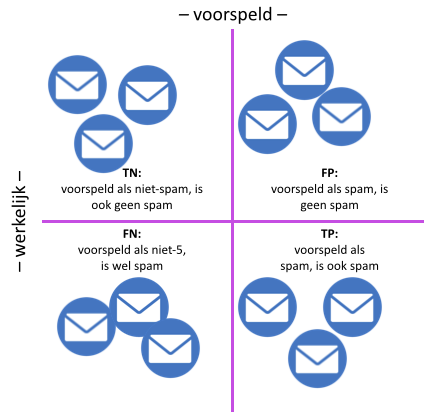
\includegraphics[width=.75\textwidth]{conf_matrix}
\caption{Een voorbeeld van een \textit{confusion matrix}.\label{img:conf_matrix1}}
\end{figure}

Berichten die correct zijn geclassificeerd als niet-spam, noemen we \textit{terechte negatieven} (Engels: \textit{true negative}); berichten die zijn geclassificeerd als niet-spam, maar wel spam zijn heten \textit{foutnegatieven} (Engels: \textit{false negative}). Omgekeerd noemen we berichten die werkelijk spam zijn en ook als zodanig zijn geclassificeerd \textit{terechte positieven} (Engels: \textit{true positive}) en berichten die als spam zijn geclassificeerd maar dat niet zijn \textit{foutpositieven} (Engels: \textit{false positive}). In de matrix in figuur \ref{img:conf_matrix1}, en in de berekeningen hieronder, worden deze waarden aangeduid met $TN$, $FN$, $TP$ en $FP$, respectievelijk.

Een perfecte classificeerder zou alleen terechte positieven en terechte negatieven hebben, zonder fouten. De confusion matrix van zo'n classificeerder zou dus gelijk zijn aan een diagonaalmatrix – alleen niet-nul waarden wanneer $i \neq j$. Voor de nagenoeg alle classificeerders is dit echter een onhaalbare kaart.

\subsection{Precisie en sensitiviteit}
Doordat we in de confusion matrix de correcte en de incorrecte voorspellingen in één overzicht hebben, kunnen we hier veel informatie uit destilleren. Niet alleen de individuele cijfers, maar juist de \textit{verhouding} hiertussen is van belang. Zo kunnen we iets zeggen over de accuratesse van de classificeerder door te kijken naar hoeveel van de voorspelde waarden ($TP+FP$) ook daadwerkelijk die waarde hebben ($TP$). Deze metriek heet de \textit{precisie} (Engels: \textit{precision}, ook wel \textit{positive predictive value} of \textit{PPV}):

\[
  PPV = \frac{TP}{TP+FP}
\]

Je kunt natuurlijk een PPV hebben van honderd procent verkrijgen door je te focussen op slechts één positieve voorspelling en je ervan te vergewissen dat deze correct is ($1/(1+0)=1$). Een dergelijke classificeerder is echter niet zo heel nuttig, omdat hij alle verdere observaties negeert. Hierom wordt de precisie in de regel gecombineerd met de \textit{sensitiviteit} (Engels: \textit{sensitivity}, ook wel de \textit{recall} of de \textit{true positive rate} of TPR genoemd): de verhouding tussen de correct geclassificeerde observaties en het totaal aantal observaties dat werkelijk tot die klasse behoort:

\[
  TPR = \frac{TP}{TP+FN}
\]

Het is vaak handig om de verhouding tussen de precisie en de sensitiviteit in één waarde uit te kunnen drukken, bijvoorbeeld wanneer je meerdere classificeerders eenvoudig met elkaar wilt vergelijken. Hiervoor wordt de zogenaamde F1-score gebruikt: het harmonisch gemiddelde van de precisie en de sensitiviteit.

\[
\begin{aligned}
  F_1 &= 2 \times \frac {\text{precisie}\times\text{sensitiviteit}}{\text{precisie}+\text{sensitiviteit}}\\
 &= \frac {TP}{TP+\frac{FN+FP}{2}}
\end{aligned}
\]

Zoals je kunt nagaan is de F1 score beter naarmate de PPV en de TPR dichter bij elkaar komen te liggen. Er bestaat echter een afruil tussen de PPV en de TPR: je kunt geen classificeerder maken die zowel een hoge PPV als een hoge TPR heeft. Welke van deze twee je belangrijker vindt, is een keuze die samenhangt met het domein en de functie van je systeem. Als je bijvoorbeeld een netwerk wilt trainen dat video's van dierenmishandeling opzoekt, is de sensitiviteit belangrijker dan de precisie – je krijgt dan wel een paar keer onterecht een melding van een foute video (lage precisie), maar je haalt wel de meeste daadwerkelijk foute video's eruit (hoge sensitiviteit). Omgekeerd kun je een netwerk maken dat bepaalt of een video geschikt is voor jonge kijkers. In dat geval heb je waarschijnlijk liever een systeem dat af en toe geschikte video's afkeurt (lage sensitiviteit), zolang het maar zoveel mogelijk slechte video's filtert (hoge precisie). 

\subsection{Andere waarden}
Van belang zijn verder nog de \textit{negatief voorspellende waarde}, de \textit{foutnegatieve verhouding} en de \textit{foutposieve verhouding}. Net als de positief voorspellende waarde zegt de negatief voorspellende waarde (Engels: \textit{NPV}) iets over de verhouding tussen de voorspelde negatieve waarden en het totaal aantal werkelijke negatieve waarden. Ook de keuze of je de PPV of de NPV zwaarder vindt wegen hangt af van het domein en het doel van je systeem. Is de positieve voorspellende waarde belangrijker dan de negatieve, of juist andersom? Bijvoorbeeld in het geval van ziekte-indicaties kan dit veel uitmaken.

De foutnegatieve en foutpositieve verhoudingen (Engels: \textit{False Negative Rate}, \textit{FNR} en \textit{False Positive Rate}, \textit{FPR}, respectievelijk) zijn eenvoudig de waarden van de foutief geclassificeerde observaties ten opzicht van het totaal. 

\[
\begin{aligned}
FNR &= \frac{FN}{FN+TP}\\
FPR &= \frac{FP}{FP+TN}
\end{aligned}
\]

Hoewel er nog meer verhoudingen en metrieken uit de confusion matrix te identificeren zijn, volstaan degene die hierboven besproken zijn wel om een goede en objectieve vergelijking tussen verschillende systemen en classificeerders mogelijk te maken.

